\documentclass{article}

% if you need to pass options to natbib, use, e.g.:
%     \PassOptionsToPackage{numbers, compress}{natbib}
% before loading neurips_2018

% ready for submission
% \usepackage{neurips_2018}

% to compile a preprint version, e.g., for submission to arXiv, add add the
% [preprint] option:
%     \usepackage[preprint]{neurips_2018}

% to compile a camera-ready version, add the [final] option, e.g.:
\usepackage[final]{projects}

% to avoid loading the natbib package, add option nonatbib:
%\usepackage[nonatbib]{neurips_2018}

\usepackage[utf8]{inputenc} % allow utf-8 input
\usepackage[T1]{fontenc}    % use 8-bit T1 fonts
\usepackage{hyperref}       % hyperlinks
\usepackage{url}            % simple URL typesetting
\usepackage{booktabs}       % professional-quality tables
\usepackage{amsfonts}       % blackboard math symbols
\usepackage{nicefrac}       % compact symbols for 1/2, etc.
\usepackage{microtype}      % microtypography
\usepackage{amsmath}
\usepackage{graphicx}
\usepackage{dsfont}
\usepackage{subcaption}
\usepackage{MnSymbol}%
\usepackage{wasysym}%

\usepackage{mathtools}

\usepackage[ruled]{algorithm2e}

\newtheorem{theorem}{Theorem}
\newtheorem{definition}{definition}
\newtheorem{lemma}{Lemma}
\newtheorem{proof}{Proof}[section]




\title{"Policy Iteration" through evolutionary of Augmenting Topology}

\author{%
  Yunian Pan \\
  Department of Electrical Engineering \\ 
  \texttt{yp1170@nyu.edu} 
}

\begin{document}

\maketitle

\begin{abstract}
  This report presents the project which follows the instructions of the paper "Evolutionary Function Approximation for Reinforcement Learning" $^{[1]}$ to do some
  simulations of reinforcement task using the related algorithm. 
  
  In the context that we have been using deep learning that in most real-world reinforcement learning tasks, 
TD methods require a function approximator to represent the value function. However, using function approximators
 requires manually making crucial representational decisions, our goal is to develop the algorithm to automate the search for 
 best function representations.
 


\end{abstract}

\section{Introduction}
TD methods have been conceived as well-established algorithms that can handle reinforcement learning tasks, when the problem scale is not large, the value function can be represented as a table of state-action pairs, but for large scale systems or for problems that has infinite dimension of 
state space or action space, it remains problematic to only use a "table", instead the function approximator which represents the mapping from state-action pairs to values via a more concise,
parameterized function and uses supervised learning methods to set its parameters, plays an important role where we can omit the step of enumering over
the state-action space.

However, using function approximators requires making crucial representational decisions (e.g. the number of hidden units and initial weights of a neural network. 
Poor design choices can result in estimates that diverge from the optimal value function and agents that perform poorly. Even for reinforcement learning algorithms 
with guaranteed convergence, achieving high performance in practice requires finding an appropriate representation for the function approximator. 

Section 2 will present the background including Q-learning and deep Q-learning, genetic algorithms and NEAT framework and NEAT algorithm for reinforcement learning and some basic related experiments;
Section 3 will have some discussion over the results obtained from the experiments.

\section{Background}
This section mainly contains two parts, one is for the development of Q-learning, Deep Q learning, and some variance of them; The another will discuss the NEAT
machinery, framework and using NEAT to do reinforcement learning, specifically, we will start from the general framework of genetic algorithm and with a little bit discussion
on how it works, then introduce a gene encoding scheme that NEAT relies on.
\subsection{Q-learning}

In the tabular case, the algorithm is defined by the following update rule, applied each time the agent transitions from state s to state $s^{\prime}$:
\begin{equation}
   Q(s,a ) = (1 - \alpha) Q(s, a) + \alpha( r + \gamma  \min_{a^{\prime}}Q(s^{\prime} ,a^{\prime}) ) \label{q}
\end{equation}
where $\alpha \in [0, 1]$ is a learning rate parameter, $\gamma \in [0, 1]$ is a discount factor, and $r$ is the immediate reward the agent receives upon taking action $a$.

This equation was initially derived from Bellman equation regarding Markov Decision Process, recall the original operator of value function:
\begin{equation}
  (TJ)(i) : = \min_{u \in U(i)} \sum_{j=1}^{n} p_{ij}(u)[g(i,u,j)+ \alpha J(j)]
\end{equation} 
define: $Q(s,a) = \sum_{j=1}^{n} p_{ij}(u)[g(i,u,j)+ \alpha J(j)]$, we can omit the probability transition, and through Robins-Monro algorithm
we solve the Q-learning problem and end up with the update rule $\ref{q}$.

 
 \subsection{Q-Learning with NN}

 Particularly when combined with neural network function approximators, 
 algorithm $\ref{1}$ describes the Q-learning algorithm using a neural network to approximate the value function.  
   The parameter $\lambda$ the sample roll-out cost decay, which is for the convenience of
  doing $TD(\lambda)$ extension, which we usually set to 0 or 1, respectively representing the value iteration method and the policy evaluation method.

   \begin{algorithm}[H] 
     \caption{Deep Q-Learning}
     \label{1}
     \KwIn{$S:$ set of all states; $A:$ set of all actions; 
     $\alpha:$ learning rate; $\gamma:$ discount factor; $\lambda:$ eligibility decay rate; 
     $\epsilon_{td}:$ exploration rate; $e:$ total number of episodes;}
     \textbf{Initialize:} $N \leftarrow$ INIT-NET$(S,A)$ \;    
     \For{ $i \leftarrow 1 $ to $e$ }{$s, s^{\prime} \leftarrow $ null, INIT-STATE($S$)\;
     \While{Terminal-state?(s)}{
       $Q[] \leftarrow $EVAL-NET$(N,s^{\prime})$\;
       \textbf{With-prob}($\epsilon_{td}$) $a^{\prime} \leftarrow$ RANDOM$(A)$\;
       \textbf{else:} $a^{\prime} \leftarrow \arg\max Q[j]$\;
       \eIf{$s \neq null $}
       {BACKPROP$(N,s,a,(r + \gamma \max_{j} Q[j])/ \alpha, \gamma, \lambda)$ \;}
       {$s, a \leftarrow s^{\prime}, a^{\prime}$\;
       $r, s^{\prime} \leftarrow$ TAKE-ACTION$(a^{\prime})$}
     }
     }
    \end{algorithm}

\subsection{NEAT}
\subsubsection{genetic algorithm}

Genetic algorithm(GA) is a metaheuristic inspired by the process of natural selection that belongs to the larger class of evolutionary algorithms(EA).
Genetic algorithms are commonly used to generate high-quality solutions to optimization and search problems by relying on bio-inspired operators such as mutation, crossover and selection.$^{[3]}$

The flow chart $\ref{flow}$ describes the standard evolution scheme:
\begin{figure}[htbp]
  \centering
  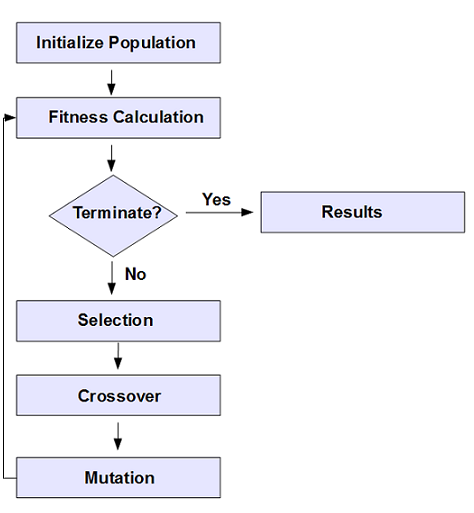
\includegraphics[width = .5\textwidth]{genetic}
  \caption{from Google Image}
  \label{flow}
\end{figure}
Inspired by the framework, one might think about apply it to finding the best structure of a neural network. 


\subsubsection{Genetic encoding}

In order to develop the neural evolution algorithm, we need a standard method to encode the neural networks as genotypes so that we can
do crossover and mutation operation based on the genotypes provided. NEAT encodes the neural networks in following aspects:

Genomes in NEAT are linear representations of network connectivity. The figure $\ref{genotype}$ illustrates a genotype to phenotype mapping example. 

\begin{figure}[htbp]
  \centering
  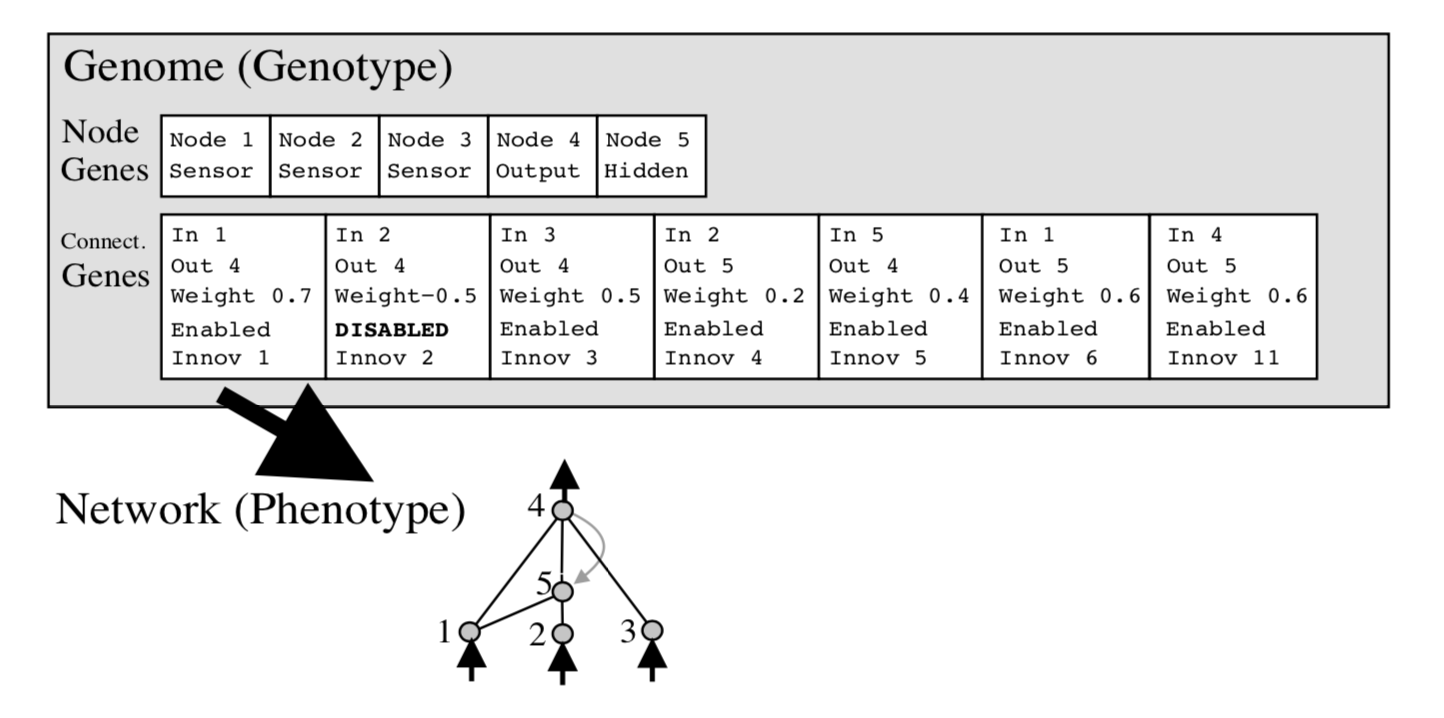
\includegraphics[width = .6\textwidth]{genome}
  \caption{genotype and phenotype from $^{[2]}$}
  \label{genotype}
\end{figure}

The figure $\ref{crossover}$ illustrates Matching up genomes for different network topologies using innovation numbers. 
 \begin{figure}[htbp]
  \centering
  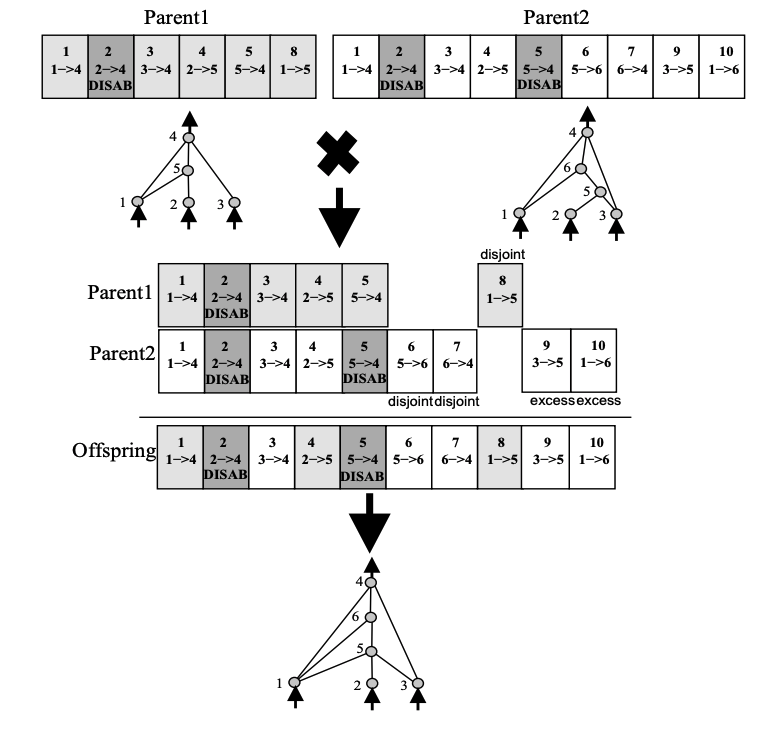
\includegraphics[width = .75\textwidth]{crossover}
  \caption{crossover from $^{[2]}$}
  \label{crossover}
\end{figure}

Figure $\ref{mutation}$ illustrates the two types of structural mutation in NEAT. 
   
\begin{figure}[htbp]
    \centering
    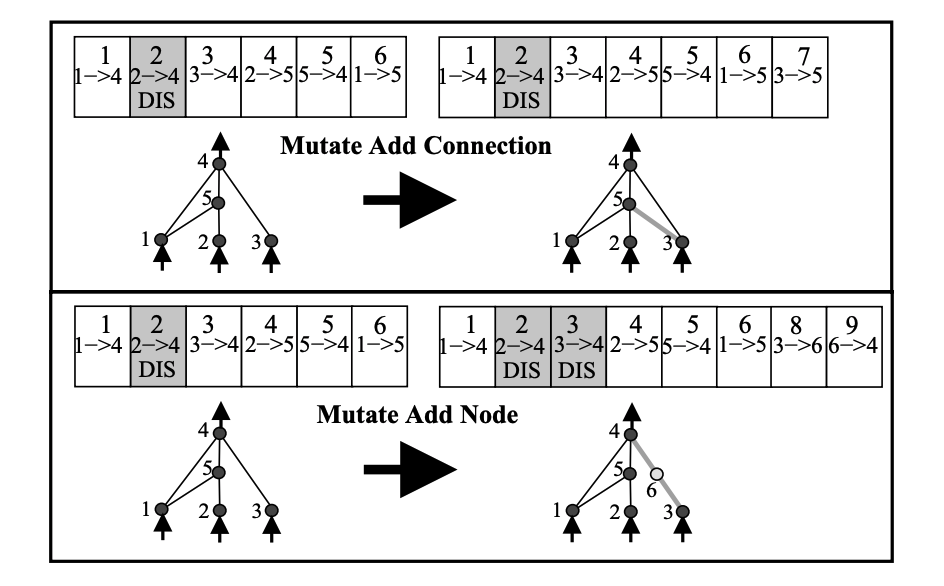
\includegraphics[width = .75\textwidth]{mutation}
    \caption{mutation from $^{[2]}$}
    \label{mutation}
  \end{figure}


\subsubsection{NEAT algorithm}
Without the aid of TD methods, namely Q-learning, NEAT can tacle reinforcement learning in that NEAT does not attempt to learn a value function but tries to find good policies directly by training action selectors,
which map states to the action the agent should take in that state, as the same as we do in policy evaluation reinforcement learning, which uses the global optimizing 
techniques that directly search the space of potential policies.

Algorithm $\ref{neat}$ contains a high-level description of the NEAT algorithm applied to an episodic reinforcement learning problem. It differs from 
the original algorithm in that for every step of choosing network for policy evaluation, the network is not chosen from directly the fixed order of
population vector, but randomly selected. This change does not significantly alter NEAT’s behavior but facilitates to excel online by balancing exploration and exploitation within and across generations.

\begin{algorithm}[H]
  \label{neat}
  \caption{NEAT($S, A, p , m_n, m_l, g, e$)}
  \KwIn{$S$:set of all states, $A$:set of all actions, $p$:population size , $m_n$: rate of adding node, $m_l$: rate of adding link, $g$: generations, $e$: episodes;}
  \textbf{Initialize:} $P[] \leftarrow$ Init-Populations$(S,A,p)$ \;    
  \For{ $i \leftarrow 1 $ to $g$ }{\For{$j \leftarrow 1 $ to $e$}{
  $N, s, s^{\prime} \leftarrow $ Random($P$), null, INIT-STATE($S$)\;
  \While{Terminal-state?(s)}{
    $Q[] \leftarrow  $EVAL-NET$(N,s^{\prime})$\;
    $a^{\prime} \leftarrow \arg\max Q[j]$;  $\quad$
    $s, a \leftarrow s^{\prime}, a^{\prime}$;  $\quad$
    $r, s^{\prime} \leftarrow$ TAKE-ACTION$(a^{\prime})$\;
    $N.fitness \leftarrow N.fitness + r$
    }
    $N.episodes \leftarrow N.episodes + 1$
    }
  $P^{\prime} \leftarrow$ new array of size p\;
  \For{$j \leftarrow 1 $ to $p$}{
    $P^{\prime}[] \leftarrow$  Breed-Net$(P[])$\;
    \textbf{with-probability} $m_n$: ADD-Node-Mutation($P^{\prime}[j]$)\;
    \textbf{with-probability} $m_l$: ADD-link-Mutation($P^{\prime}[j]$)
  }
  $P[] \leftarrow P^{\prime}[]$
  }
  \end{algorithm}


NEAT speciates the population, in order to avoid that adding new structure to a network might initially reduces its fitness.
  so that individuals compete primarily within their own niches rather than with the population at large.






\subsection{Comparisons}
Several comparisons regarding the comparisons between different version of algorithms are listed in this section:









 
\section{Simulations and comparison}
There are some of the results demonstrated with an emphasis on NEAT algorithm.

\subsection{Mountain car}

Starting from the simplest case, the first environment we tested is the Mountain car, just as the paper has presented,
\begin{figure}[htbp]
  \centering
  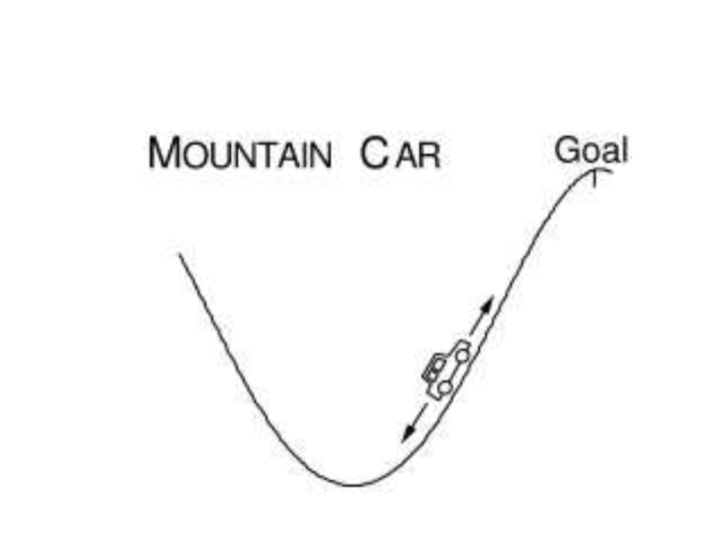
\includegraphics[width = .4\textwidth]{Mountaincar}
  \caption{Mountain car from Sutton(1998)}
  \label{mc}
 \end{figure}
As $\ref{mc}$ illustrates, the car which is stuck in the valley doesn't have enough power to drive to the goal, instead it has to drive to the left hill
in order to build some inertia and reach the goal leveraging the speed it obtains.

\subsubsection{Q-learning}

As a counterpart, when manually determine the neural network using tensorflow with 811 total parameters, the mountain car task remains problematic after 1000 episodes of training, the episode reward 
keeps at -200 in the current used OpenAI gym environment, to achieve better results the exploration rate annealing was implemented. the test results will be covered in the video, the learning curve will not be provided here since it's
a straight horizontal line. 

\subsubsection{NEAT}

 Table $\ref{table1}$ shows some basic configuration parameters that was used for NEAT(still some others not listed).
 \begin{table}[htbp]
  \centering
  \caption{parameter setting}
  \label{table1}
  \centering
  \begin{tabular}{llllll}
    \toprule
    %\multicolumn{5}{c}{}                   \\
    \cmidrule(r){1-6}
    state & action &   node bias  &  compa-threshold   & stagnation     &  sp-elitism   \\
    \midrule
   2  & discrete(3) & [-30,30]  & 3.0 & 15 &  4    \\
   \cmidrule(r){1-6}
   pop size & mutation rate & Node-add/delete    & Connect-add/delete    & activation & elitism  \\
    \midrule
   150 & $0.1$ &  $0.9/0.2$  & $0.4/0.1$ & relu &  2    \\
        \bottomrule
  \end{tabular}
\end{table}

As $\ref{learn1}$ shows, we are able 
 to find the best individuals from the population within the 60 generations, at the very beginning the performance is poor, but once there are 
 some "good" mutations happening, the next generation will improve by inheriting these nice topologies. 
\begin{figure}[htbp]
  \centering
  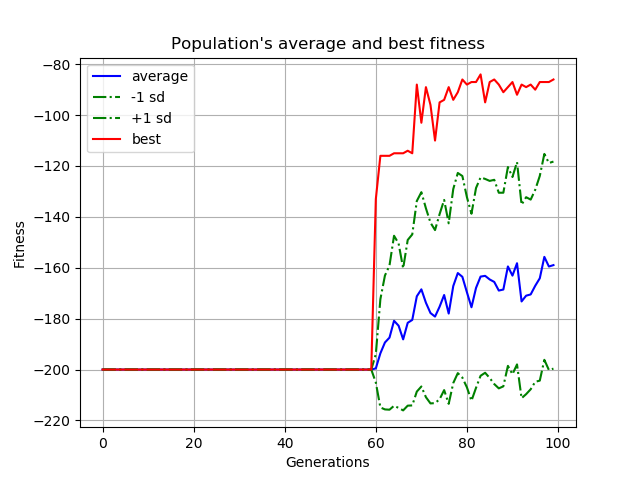
\includegraphics[width = .7\textwidth]{mountaincarlearningcurve}
  \caption{Learning curve of mountain car}
  \label{learn1}
 \end{figure}
The final winner's structure is as shown in $\ref{evo1}$,

 \begin{figure}[htbp]
  \centering
  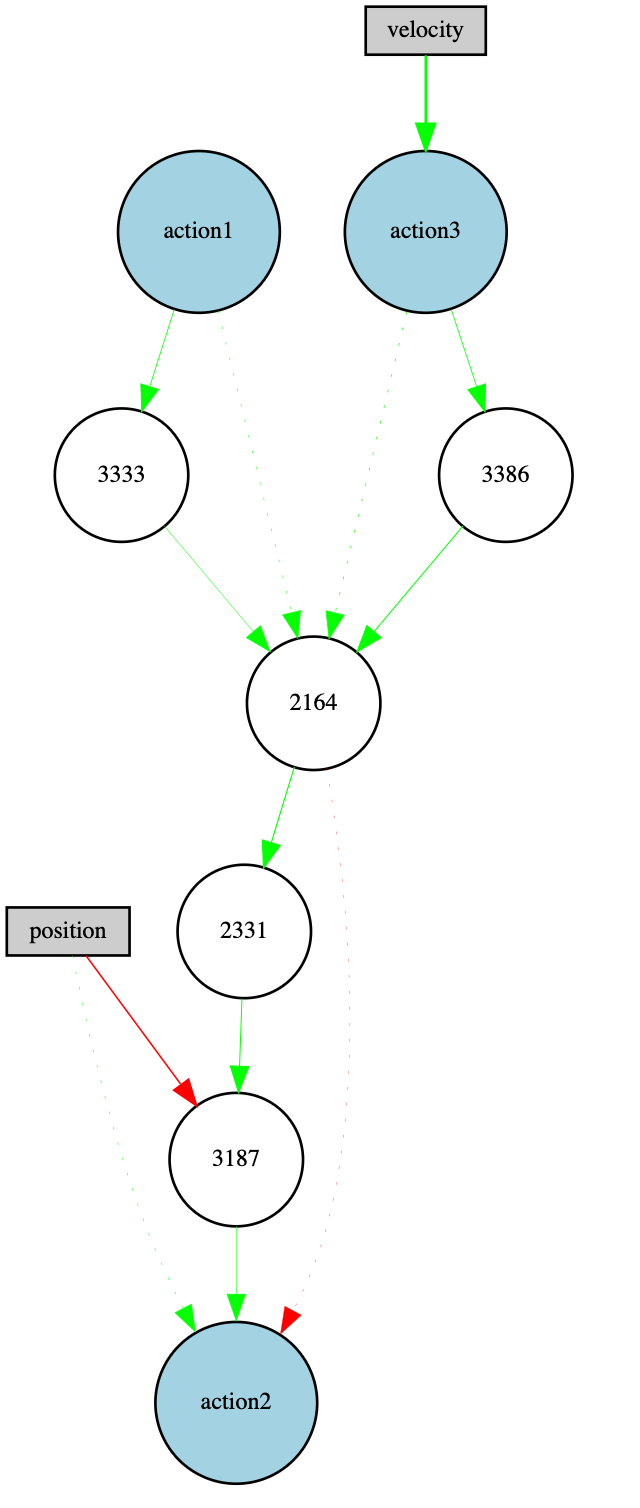
\includegraphics[width = .3\textwidth]{mountaincarnetwork}
  \caption{Final conectivity of mountain car, the network is allowed to become recurrent as we add nodes and connections}
  \label{evo1}
 \end{figure}

 $\ref{spe1}$ demonstrates the speciation evolution, genomes that with genome distance less than compatibility threshold 3 would be considered
 one species.

 \begin{figure}[htbp]
  \centering
  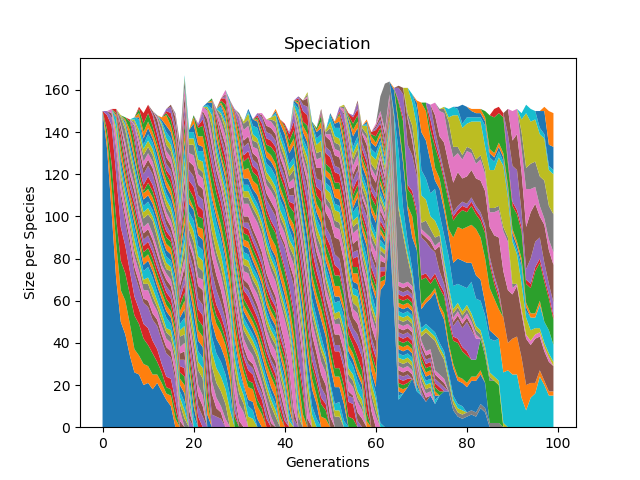
\includegraphics[width = .7\textwidth]{mountaincarspecies}
  \caption{Species evolution}
  \label{spe1}
 \end{figure}



\subsection{Atari game: AirRaid}
An environment with larger complexity called AirRaid has also been tested using the both Q-learning and NEAT algorithm.

\subsubsection{Q-learning}
Manually determined neural network has 297,478 parameters, during the exploration steps, the model might have achieved greater score 
higher than 1000 but overall the learning curve has been stuck in somewhere. Using the same algorithm as before in the mountain car task, still it has a bad performance.

\begin{figure}[htbp]
  \centering
  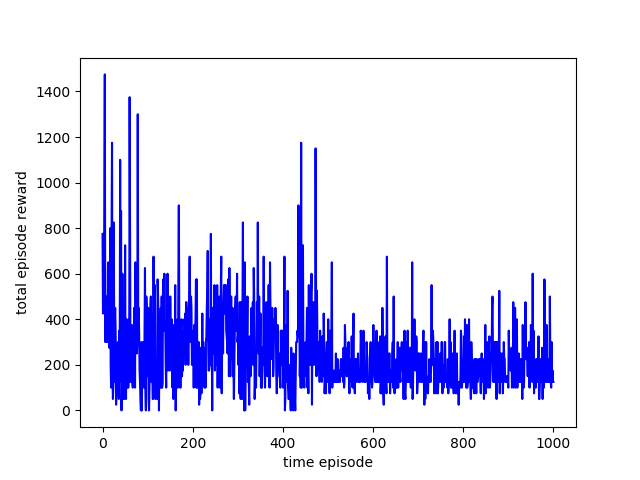
\includegraphics[width = .7\textwidth]{airq}
  \caption{Learning curve of AirRaid Q-learning}
  \label{learnq}
 \end{figure}



\subsubsection{NEAT}
Table $\ref{table2}$ shows the basic configuration of
neat algorithm:
\begin{table}[htbp]
  \centering
  \caption{parameter setting}
  \label{table2}
  \centering
  \begin{tabular}{llllll}
    \toprule
    %\multicolumn{5}{c}{}                   \\
    \cmidrule(r){1-6}
    state & action &   node bias  &  compa-threshold   & stagnation     &  sp-elitism   \\
    \midrule
   128  & discrete(6) & [-30,30]  & 3.0 & 15 &  4    \\
   \cmidrule(r){1-6}
   pop size & mutation rate & Node-add/delete    & Connect-add/delete    & activation & elitism  \\
    \midrule
   150 & $0.1$ &  $0.9/0.2$  & $0.4/0.1$ & relu &  2    \\
        \bottomrule
  \end{tabular}
\end{table}

After 100 generations of training, each generation contains variant episodes within which my action in the environment will be finished,
learning curve is just shown in Figure $\ref{learn2}$.

\begin{figure}[htbp]
  \centering
  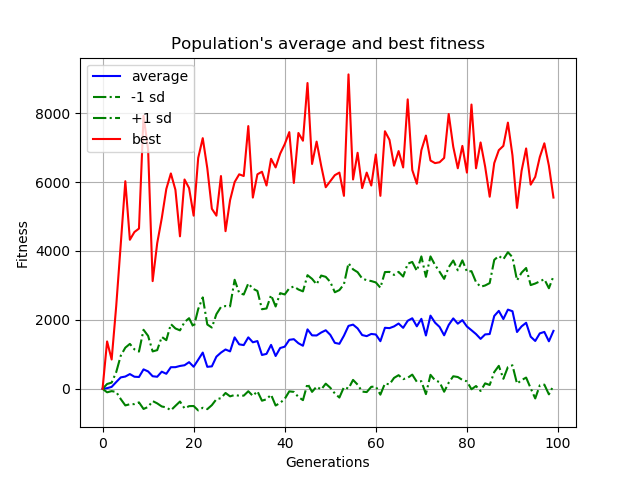
\includegraphics[width = .7\textwidth]{first100}
  \caption{Learning curve of AirRaid}
  \label{learn2}
 \end{figure}

 \begin{figure}[htbp]
  \centering
  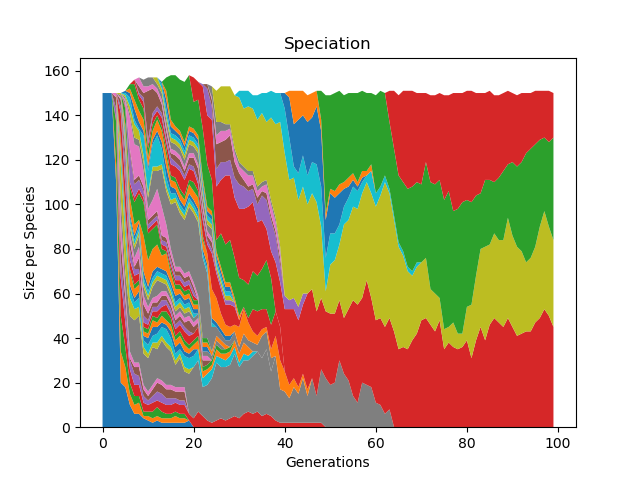
\includegraphics[width = .7\textwidth]{first100species}
  \caption{Evolution diagram of AirRaid}
  \label{evo2}
 \end{figure}
 Limited by the scale of graph, the connectivity will not shown here. As we continue breeding the networks, it will exceed the fitness threshold and stop training as we have defined
 in the configuration file,
 as shown in $\ref{learn3}$.
 \begin{figure}[htbp]
  \centering
  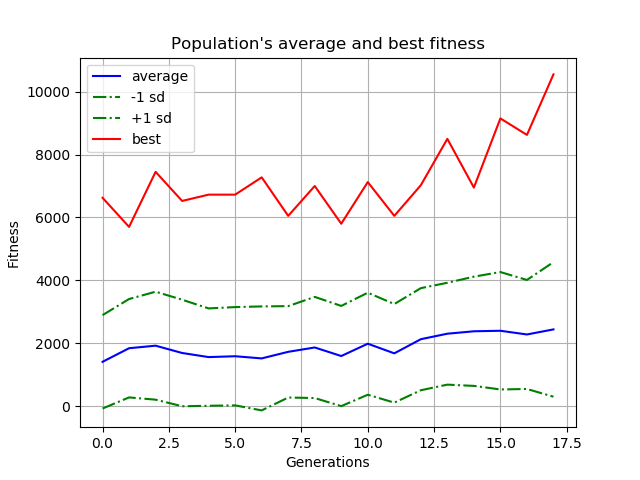
\includegraphics[width = .7\textwidth]{threshold}
  \caption{Learning curve of AirRaid}
  \label{learn3}
 \end{figure}

 


 



\section{Conclusion}

Having evidences listed before, we can summarize that :
\begin{itemize}
  \item NEAT outperform Q-learning in episodes, Generally, NEAT+Q can even perform better as shown in the mountain car and server job scheduling domain of the original paper; 
  \item NEAT explore the function representation automatically, similar to exploring a better policy, the episodes of ficticious play is equivalent to what we do during policy evaluation,
  only different in that the policy is hidden beneath the represented function of neural network, and we have multiple choice when it comes to policy update.
  \item It's safe to anticipate that some other Methods(DDQN and Duel QN) can be combined with NEAT, but in order to in corporate with those tools we have to add properties to the existing NEAT system
  so that it can perform backpropagation.
  \item  although the training process might work in some deterministic systems, it is still challenging to tacle non-stationary environment as the action selector only take 
  the current states into consideration, whether the algorithm is adaptive to the non-stationary environments or not remains to be verified.
\end{itemize}


\section*{References}

\small

[1] Whiteson, Shimon, and Peter Stone. "Evolutionary function approximation for reinforcement learning." Journal of Machine Learning Research 7.May (2006): 877-917.

[2] Stanley, Kenneth O., and Risto Miikkulainen. "Efficient reinforcement learning through evolving neural network topologies." Proceedings of the 4th Annual Conference on Genetic and Evolutionary Computation. Morgan Kaufmann Publishers Inc., 2002.

[3] Mitchell, Melanie. An introduction to genetic algorithms. MIT press, 1998.

\end{document}